\renewcommand{\NomeBloco}{Transmition Gate}
\renewcommand{\NomePTab}{tab_\NomeBloco}
\renewcommand{\NomeSTab}{tab_\NomeBloco2}
\renewcommand{\NomePFig}{fig_\NomeBloco}
\renewcommand{\NomeSFig}{fig_\NomeBloco2}
\renewcommand{\NomeTTab}{tab_\NomeBloco3}

\subsection{\NomeBloco}

O bloco \NomeBloco{} funciona como uma chave, permitindo ou n\~ao o sinal de um lado passar ao outro. O bloco apresenta as defini{\c c}\~oes de sinais de entrada e sa\'ida referidos na \autoref{\NomeSTab}.

\begin{table}[htbp]
\caption{Sinais do bloco \NomeBloco}
\label{\NomeSTab}
\centering
\begin{tabular}{ccl}

    \toprule
    Sinal & Tipo    & Descri{\c c}\~ao        \\
    \midrule \midrule
    A & Bidirecional & Sinal bidirecional 1\\
    \midrule
    B & Bidirecional & Sinal bidirecional 2\\
    \midrule
    ENABLE & Entrada & Sinal de habilita{\c c}\~ao\\
    \bottomrule
\end{tabular}
\legend{Fonte: Produzido pelo autor}
\end{table}

O circuito projetado para o bloco \'e demonstrado na \autoref{\NomePFig}.

\begin{figure}[htb]
 \label{\NomePFig}
 \centering
  \begin{minipage}{0.4\textwidth}
    \centering
    \caption{Circuito CMOS projetado para o bloco \NomeBloco} \label{\NomePFig}
    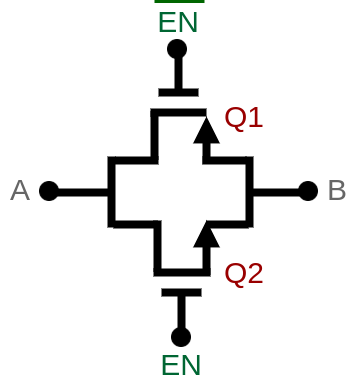
\includegraphics[scale=0.5]{Circuitos/TG.png}
    \legend{Fonte: Produzido pelo autor}
  \end{minipage}
  \hfill
  \begin{minipage}{0.4\textwidth}
    \centering
    \caption{Representa{\c c}\~ao em bloco do \NomeBloco} \label{\NomeSFig}
    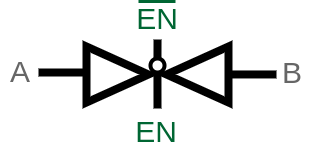
\includegraphics[scale=0.5]{Circuitos/TG_Simbolo.png}
    \legend{Fonte: Produzido pelo autor}
  \end{minipage}
\end{figure}

Os transistores utilizados no bloco \NomeBloco{} apresentam os par\^ametros mostrados na \autoref{\NomeTTab}.

\begin{table}[htbp]
\caption{Transistores do Bloco \NomeBloco}
\label{\NomeTTab}
\centering
\begin{tabular}{ccccc}
\toprule
Transistor & W ($\mu$m)  & L ($\mu$m)           & M (n° dispositivos) & S (n° dispositivos)\\
\midrule \midrule
Q1 & 0,8 & 0,18 & 1 & 1\\
\midrule
Q2 & 0,4 & 0,18 & 1 & 1\\
\bottomrule
\end{tabular}
\legend{Fonte: Produzido pelo autor}
\end{table}
\clearpage
